Question 2:\\
\textsl{Pick three hyper-parameters below and analyze how changing the hyper-parameters affect the conclusions that can be drawn from the data. Please choose at least one hyper-parameter from each of the two categories (visualization and clustering/feature selection). At minimum, evaluate the hyper-parameters individually, but you may also evaluate how joint changes in the hyper-parameters affect the results. You may use any of the datasets we have given you in this project. For visualization hyper-parameters, you may find it productive to augment your analysis with experiments on synthetic data, though we request that you use real data in at least one demonstration. $[...]$ }\\
\textsl{For visualization hyper-parameters, provide substantial visualizations and explanation on how the parameter affects the image.}\\
\textsl{For clustering/feature selection, provide visualizations and/or numerical results which demonstrate how different choices affect the downstream visualizations and feature selection quality.}\\
\textsl{Provide adequate explanations in words for each of these visualizations and numerical results.}\\

Answer:\\
Category A (visualization)\\
In the following task I will use the data from problem 1. Like before, I will move on with 50 PC's for the visualization with help of the T-SNE plot. The hyper-parameters of interest are the perplexity and the early exaggeration rate of the T-SNE function.\\

The perplexity parameter influences how the distance between individual points are set (see figure \ref{fig:TSNE_hyper_parameter}). With a high perplexity clusters start to merge into one another. In contrast, a too low perplexity results in clusters of low density. The documentation states that larger data sets require usually a larger parameter. The recommended range is between 5 and 50.\\

\begin{figure}[h]
	\centering
	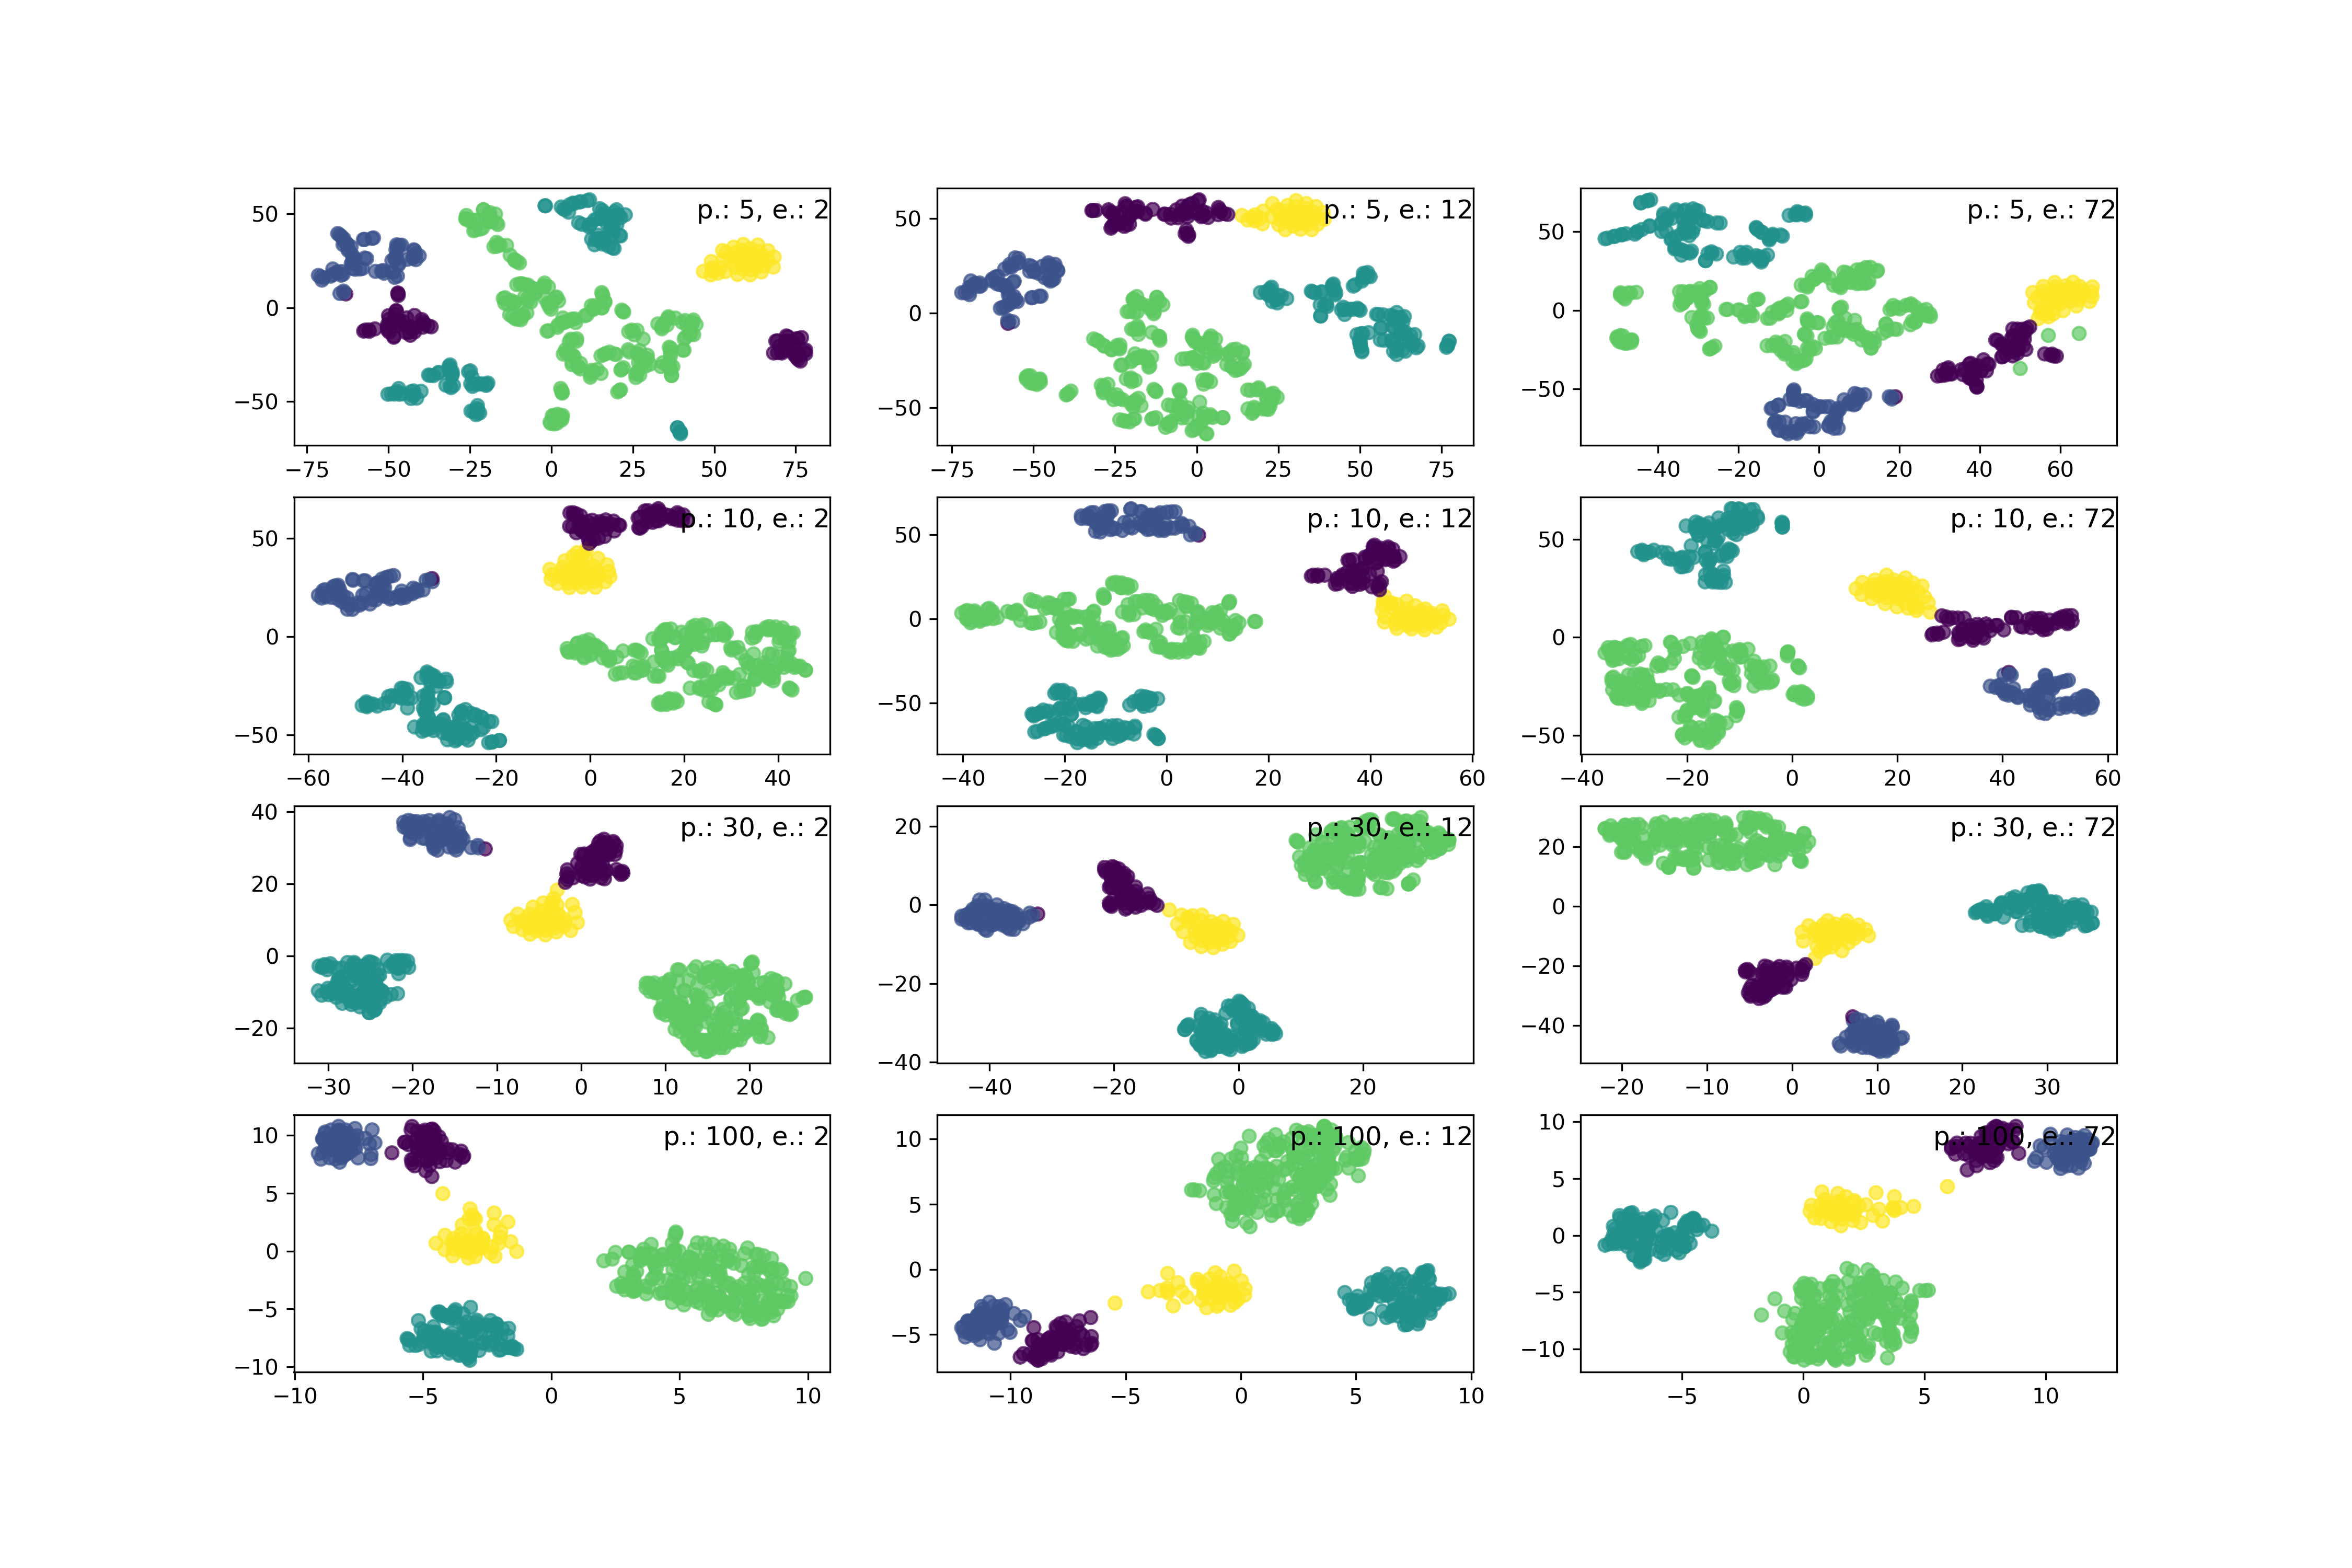
\includegraphics[width=1.0\linewidth, trim={4cm 2cm 3.5cm 2cm}]{problem_03/TSNE_hyper_parameter}
	\caption{T-SNE plots for different hyper-parameters (p: perplexity, e: early exaggeration, 50 PC's)}
	\label{fig:TSNE_hyper_parameter}
\end{figure}

According to the sklearn documentation the early exaggeration "controls how tight natural clusters in the original space are in the embedded space and how much space will be between them". By comparing the plots row-wise we can see small quality differences for constant perplexity parameters (see figure \ref{fig:TSNE_hyper_parameter}). The largest difference can be seen for a low perplexity of 5. Here the separation between the clusters for this perplexity was achieved. The default setting for this parameter is 12, which shows the best distinction between the different clusters.\\

In this comparison the best visualization was achieved with a perplexity of 30. The early exaggeration is in this case of minor weight due to comparable results.\\

\vspace{2cm}

Category B (clustering/feature selection)\\
For the next task I will use the same data set as before, but now as an unsupervised data set. Therefore I will analyze which number of clusters leads to the best results. The used tool is the K-Means algorithm.\\

The first approach is analyzing quantitative tools to estimate a reasonable number of clusters. Two different approaches are plotting the average silhouette score and the WGSS over the number of clusters (see figure \ref{fig:no_of_clusters}). The silhouette plot gives three almost equally promising number of clusters with average silhouette scores around 0.36 to 0.37 for \{3,4,5\}. Here, we want to achieve high values to assign the data points to the clusters as good as possible. The second quantitative visualization is the "elbow" plot. Here, the "elbow" is a favorable candidate for the optimal number of clusters. Namely, the cluster numbers of \{4,5,6\} are good candidates.\\

\begin{figure}[h]
	\centering
	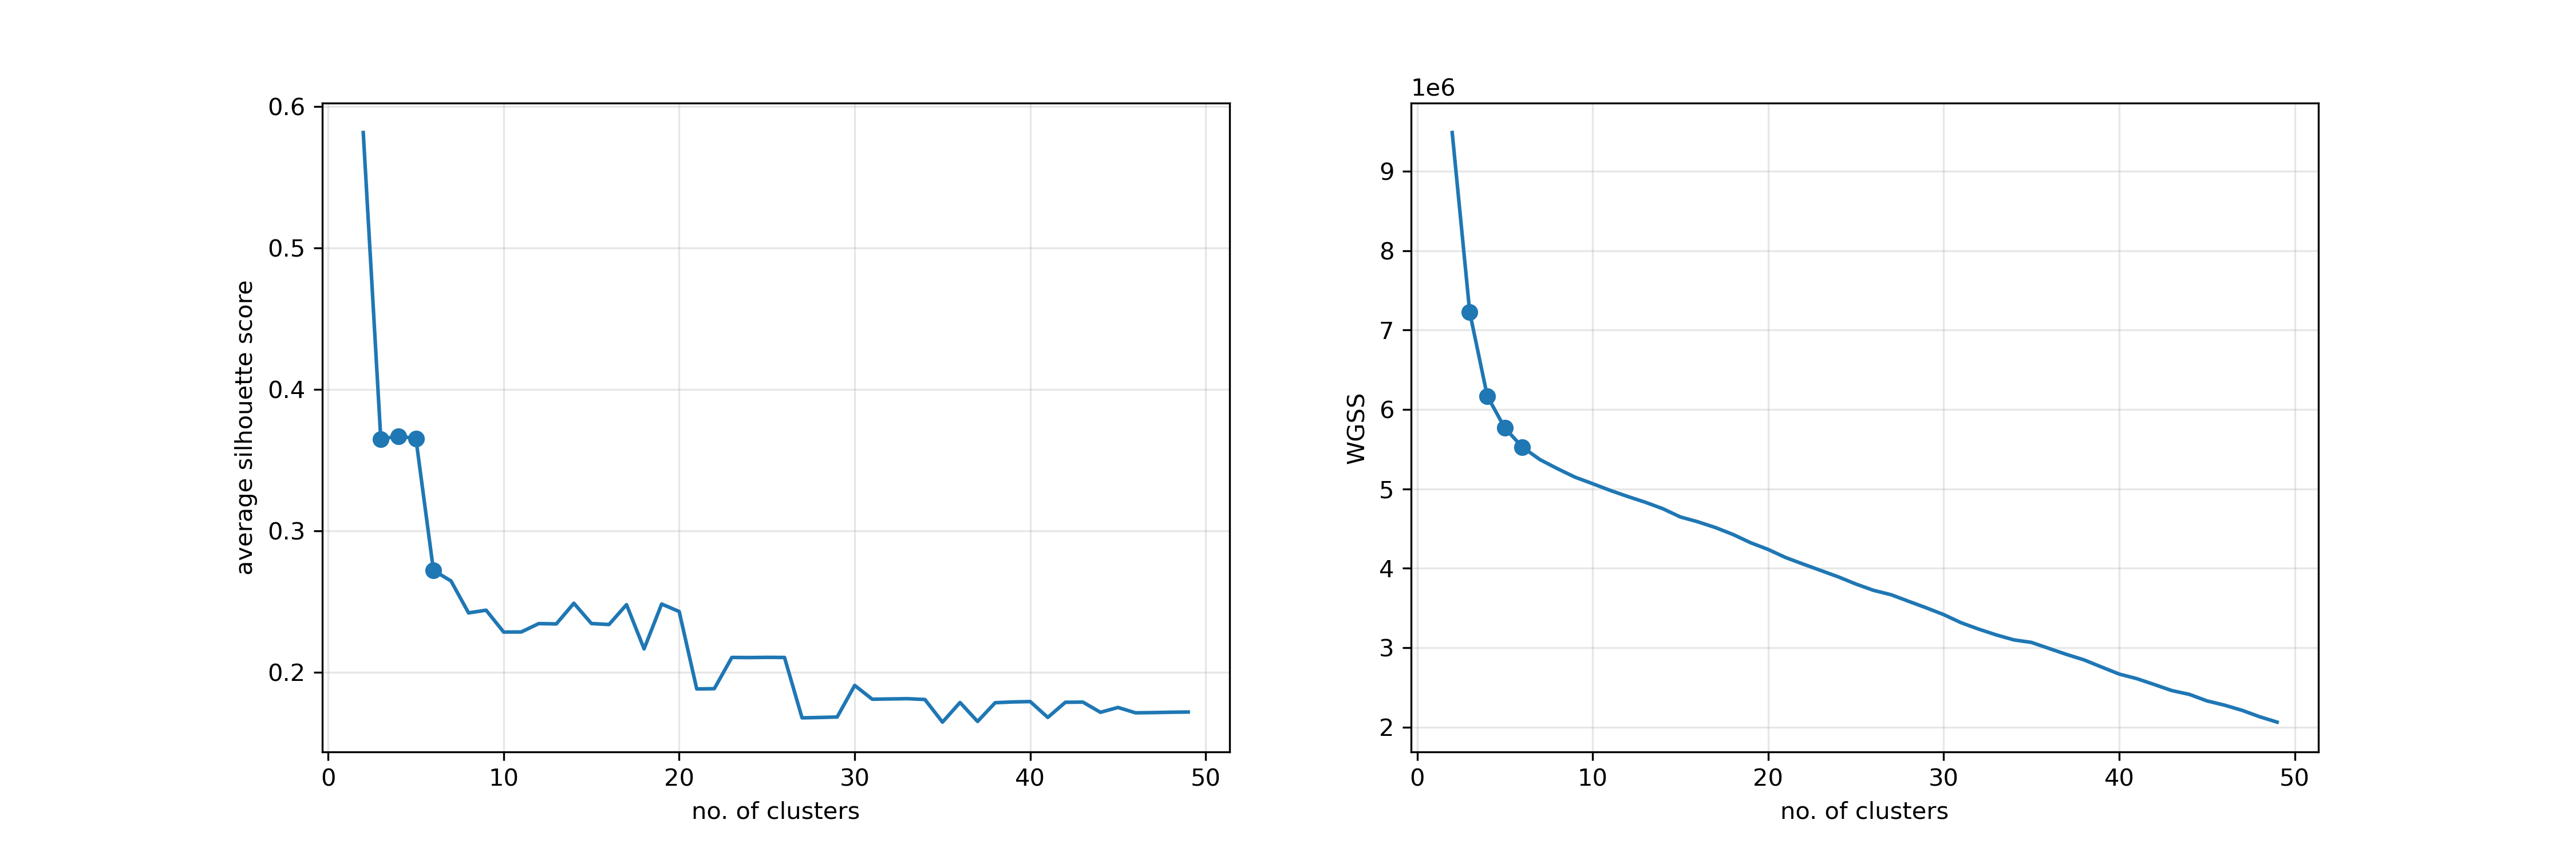
\includegraphics[width=1.0\linewidth]{problem_03/no_of_clusters}
	\caption{Silhouette and "elbow" plot (highlighted points $n=\{3,4,5,6\}$, 50 PC's)}
	\label{fig:no_of_clusters}
\end{figure}

The visualization of the clustered data points over the first two PC's leads to two different possible conclusions (see figure \ref{fig:no_of_clusters_visualization}). Without knowledge of the real number of clusters we could assume, that there are three, four or five different clusters. Each theory could be supported by the plots in figure \ref{fig:no_of_clusters} and the visualization in figure \ref{fig:no_of_clusters_visualization}.\\

\begin{figure}[h]
	\centering
	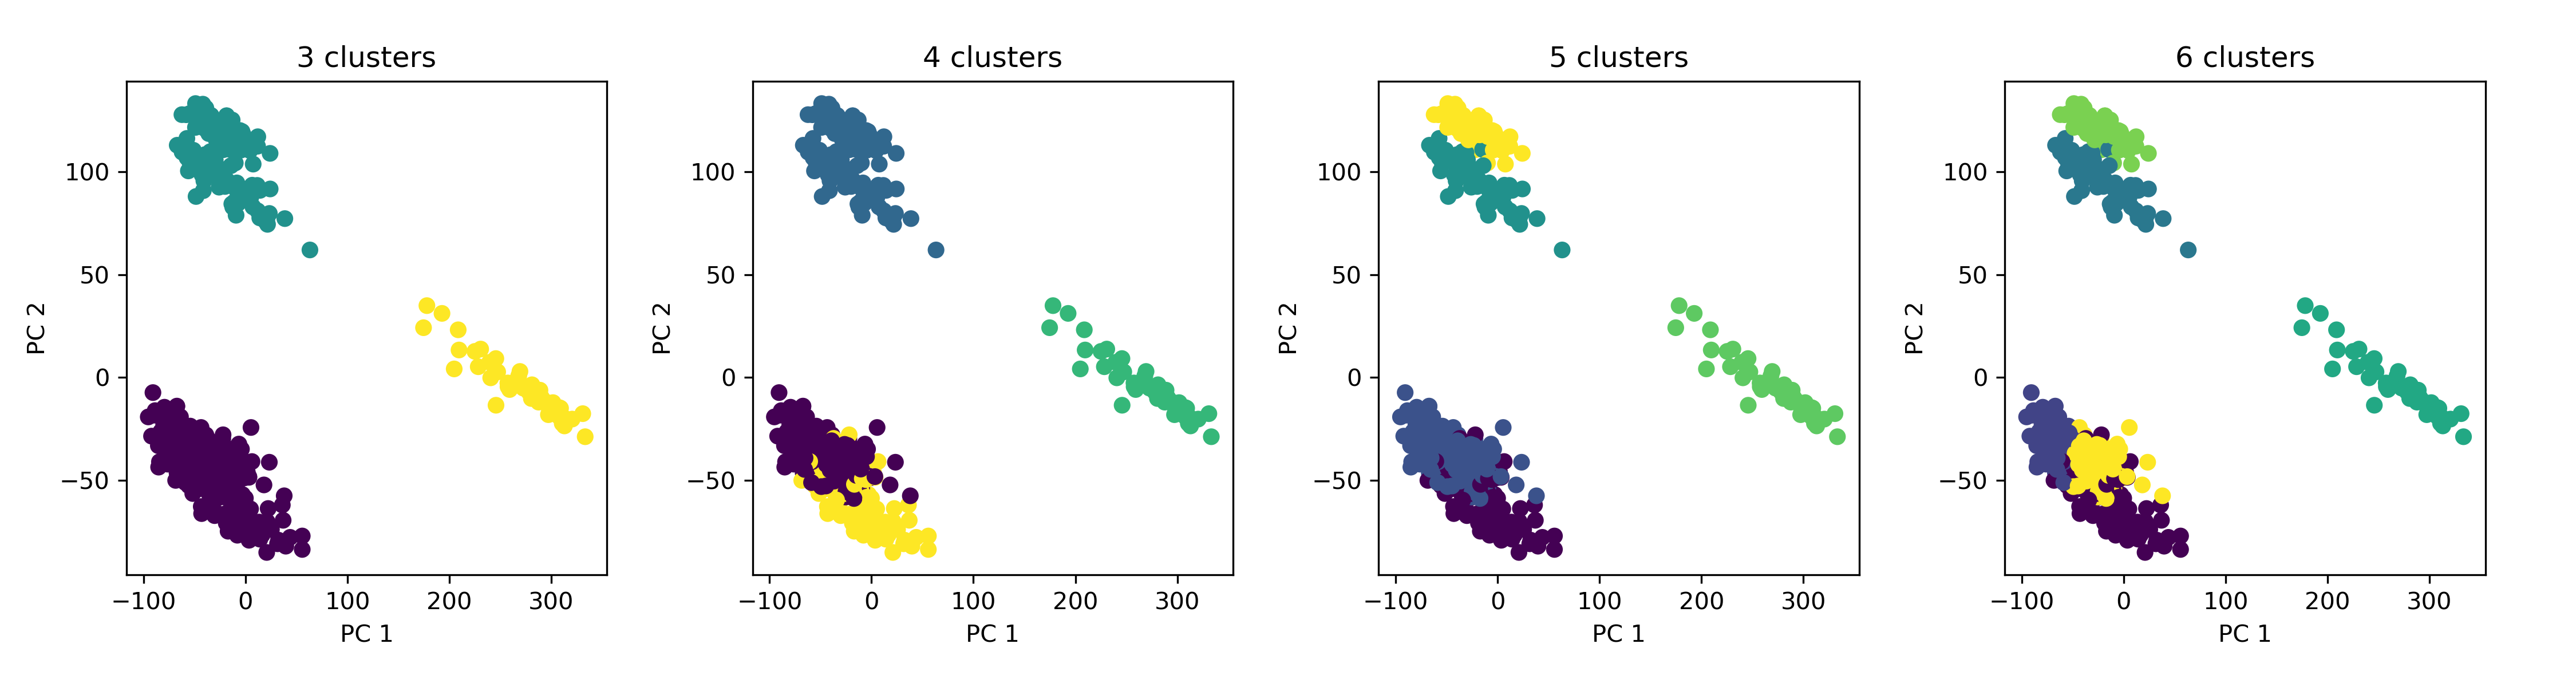
\includegraphics[width=1.0\linewidth]{problem_03/no_of_clusters_visualization}
	\caption{Visualization of clusters over the first two PC's (model used 50 PC's)}
	\label{fig:no_of_clusters_visualization}
\end{figure}

The most arguments lead to the conclusion that there are either three or five clusters. In case of three clusters, the neighbored points are assigned to one cluster with a fair space between these groups. In case of five clusters two clusters are sub-divided, which might be true as well. But in all visualizations of figure \ref{fig:no_of_clusters_visualization} there is space for subjective interpretations and therefore different decisions.\\